\documentclass[11pt,a4paper]{article}
\usepackage{amsmath}
\usepackage[english]{babel}
\usepackage{graphicx}
\usepackage{hyperref}

\begin{document}
    \begin{abstract}
        As most research papers have an abstract, there are predefined commands for telling LaTeX which part of the content makes up the abstract.
        This should appear in its logical order, therefore, after the top matter, but before the main sections of the body.
        This command is available for the document classes article and report, but not book.
    \end{abstract}

    \section{Introduction}
    Hello World!

    \section{Figures and Tables}
        Taken from \url{https://en.wikibooks.org/wiki/LaTeX/Floats,_Figures_and_Captions}.

        \begin{figure}
          \caption{A picture of a gull.}
          \centering
            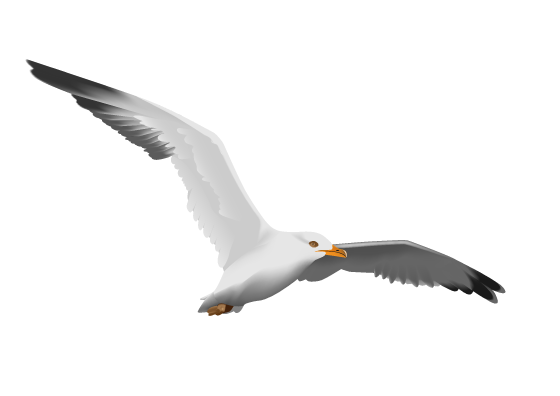
\includegraphics[width=0.5\textwidth]{gull}
        \end{figure}

        \begin{figure}
          \centering
            \reflectbox{%
              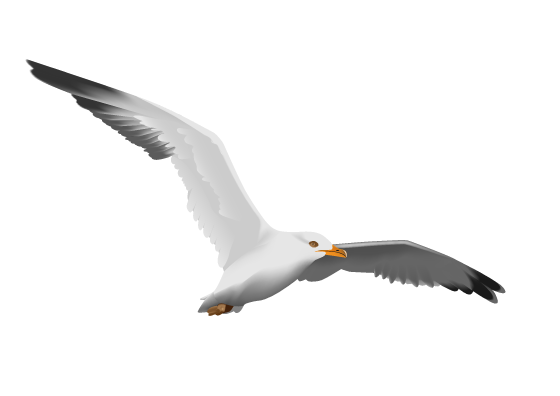
\includegraphics[width=0.5\textwidth]{gull}}
          \caption{A picture of the same gull looking the other way!}
        \end{figure}

        \begin{table}
          \centering
            \begin{tabular}{| l c r |}
            \hline
            1 & 2 & 3 \\
            4 & 5 & 6 \\
            7 & 8 & 9 \\
            \hline
            \end{tabular}
          \caption{A simple table}
        \end{table}

        Notice how the tables and figures have independent counters.

    \subsection{Math}

        \begin{equation}
            e = mc^2
        \end{equation}

        \begin{equation}
            \nabla \cdot \sigma + \mathbf{b} = \mathbf{0}
        \end{equation}

\end{document}
